\subsection{STIRLING'S EXPANSION}

Let \(x\) and \(y\) be two complex numbers not lying on the real negative half-axis; by formula (3) of VII, p.~315, with the conventions of VII, p.~316, concerning the logarithms, \(\log \Gamma(x) - \log \Gamma(y)\) is congruent modulo \(2\pi i\) to the limit of the expression

\[
(x - y) \log n + \sum_ {k = 0} ^ {n} \Big (\log (y + k) - \log (x + k) \Big).\tag{15}
\]

Let us put \(f(t) = \log(y + t) - \log(x + t)\) ; we apply the Euler-Maclaurin summation formula (VI, p.~288) to the function f:

\[
\begin{array}{l} f (0) + f (1) + \dots + f (n) = \int_ {0} ^ {n + 1} f (t) d t - \frac {1}{2} \big (f (n + 1) - f (0) \big) \\ \qquad + \sum_ {k = 1} ^ {p} \frac {b _ {2 k}}{(2 k) !} \big (f ^ {(2 k - 1)} (n + 1) - f ^ {(2 k - 1)} (0) \big) + T _ {p} (n) \end{array}
\]

with

\[
\left| \mathrm{T} _ {p} (n) \right| \leqslant \frac {4 e ^ {2 \pi}}{(2 \pi) ^ {2 p + 1}} \int_ {0} ^ {n + 1} \left| f ^ {(2 p + 1)} (u) \right| d u.\tag{16}
\]

Since

\[
f ^ {(m)} (t) = (- 1) ^ {m - 1} (m - 1)! \left(\frac {1}{(y + t) ^ {m}} - \frac {1}{(x + t) ^ {m}}\right),
\]

\(f^{(2k - 1)}(n + 1)\) tends to 0 as \(n\) tends to \(+\infty\) , for all \(k \geqslant 1\) ; it is the same for

\[
f (n + 1) = \log \left(1 + \frac {y}{n + 1}\right) - \log \left(1 + \frac {x}{n + 1}\right).
\]

Moreover, one has

\[
\int_ {0} ^ {n + 1} \log (x + t) d t = (x + n + 1) (\log (x + n + 1) - 1) - x (\log x - 1);
\]

as n tends to \(+\infty\) , one has the asymptotic expansion

\[
(x + n) \bigl (\log (x + n) - 1 \bigr) = n \log n - n + x \log n + O \left(\frac {1}{n}\right).
\]

Substituting in the expression (15) one sees finally that, as n tends to \(+\infty\) , \(\mathrm{T}_{p}(n)\) has a limit \(\mathrm{R}_{p}(x, y)\) and that one can write

\[
\log \Gamma (x) - g (x) \equiv \log \Gamma (y) - g (y) + \mathrm{R} _ {p} (x, y)\tag{mod.  \( 2\pi i \)}
\]

on putting

\[
g (x) = x \log x - x - \frac {1}{2} \log x + \sum_ {k = 1} ^ {p} \frac {b _ {2 k}}{2 k (2 k - 1)} \frac {1}{x ^ {2 k - 1}}.\tag{17}
\]

We shall now evaluate a bound for \(\mathrm{R}_{p}(x,y)\) with the help of (16), assuming that x and y are both in the subset \(H_{A}\) of C defined by the relation `` \(\mathcal{R}(z)\geqslant A\) or \(|\mathcal{I}(z)|\geqslant A\) '', where A is an arbitrary number \textgreater0 (fig.~2). To this end we remark that if \(x=s+it\) with s\textgreater A one has \(|x+u|\geqslant A+u\) for every u\textgreater0, and consequently

\[
\int_ {0} ^ {n + 1} \frac {d u}{| x + u | ^ {2 p + 1}} \leqslant \int_ {0} ^ {\infty} \frac {d u}{(\mathrm{A} + u) ^ {2 p + 1}} = \frac {1}{2 p \mathrm{A} ^ {2 p}}.
\]

Similarly, if \(|t| \geqslant A\) one has \(|x + u| = |s + u + it| \geqslant \sqrt{A^2 + (s + u)^2}\) for all real \(u\) , whence

\[
\int_ {0} ^ {n + 1} \frac {d u}{| x + u | ^ {2 p + 1}} \leqslant \int_ {- \infty} ^ {+ \infty} \frac {d u}{(\mathrm{A} ^ {2} + u ^ {2}) ^ {p + 1 / 2}} = \frac {2}{\mathrm{A} ^ {2 p}} \int_ {0} ^ {\infty} \frac {d v}{(1 + v ^ {2}) ^ {p + 1 / 2}}.
\]

Thus one sees that, when x and y are in \(H_{A}\) , one has

\[
\left| \mathrm{R} _ {p} (x, y) \right| \leqslant \frac {\mathrm{C} _ {p}}{\mathrm{A} ^ {2 p}}
\]

\pandocbounded{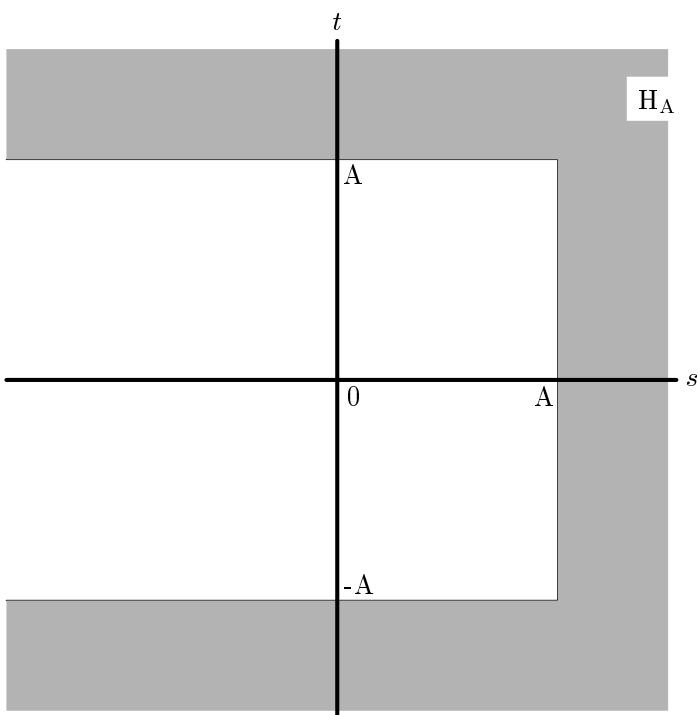
\includegraphics[keepaspectratio]{images/part002_194eed20.jpg}}\\
Fig. 2

where \(C_{p}\) depends only on p.~Now let F be the filter having the sets \(H_{A}\) as basis; the Cauchy criterion shows that, along the filter F, the function \(\log \Gamma(z) - g(z)\) has a finite limit \(\delta\) (modulo \(2\pi i\) ) and that, if one puts \(\omega(z) = \max(\mathcal{R}(z), |\mathcal{I}(z)|)\) , one has

\[
\log \Gamma (z) - g (z) - \delta \equiv O \left(\frac {1}{(\omega (z)) ^ {2 p}}\right) \pmod {2 \pi i}.\tag{18}
\]

For \(x\) real and \(> 0\) one has \(\Gamma(x) > 0\) , and \(g(x)\) is real, so one can assume that \(\delta\) is real and one has

\[
\log \Gamma (x) = g (x) + \delta + O \left(\frac {1}{x ^ {2 p}}\right).
\]

Now we shall deduce the value of the constant \(\delta\) ; by prop. 2 of VII, p.~318, applied for p = 2, one has, for real x tending to \(+\infty\)

\[
\begin{array}{c} \frac {x - 1}{2} \log \frac {x}{2} - \frac {x}{2} + \frac {x}{2} \log \frac {x + 1}{2} - \frac {x + 1}{2} + 2 \delta \\ = x \log x - x - \frac {1}{2} \log x + (\frac {1}{2} - x) \log 2 + \frac {1}{2} \log 2 \pi + \delta + o (1) \end{array}
\]

from which one deduces easily that \(\delta = \frac{1}{2}\log 2\pi\) . Finally one has the following result:

PROPOSITION 4. Along the filter \(\mathfrak{F}\) one has (for every integer \(p \geqslant 1\) ) the asymptotic expansion

\[
\begin{array}{l} \log \Gamma (z) \equiv z \log z - z - \frac {1}{2} \log z + \frac {1}{2} \log 2 \pi \\ \quad + \sum_ {k = 1} ^ {p} \frac {b _ {2 k}}{2 k (2 k - 1)} \frac {1}{z ^ {2 k - 1}} + O \left(\frac {1}{(\omega (z)) ^ {2 p}}\right) \pmod {2 \pi i} \end{array}\tag{19}
\]

(Stirling's expansion).

COROLLARY. Along the filter F one has

\[
\Gamma (z) \sim \sqrt {2 \pi} \exp (z \log z - z - \frac {1}{2} \log z).\tag{20}
\]

In particular, for \(x\) real tending to \(+\infty\) the formula (20) can be written

\[
\Gamma (x) \sim \sqrt {2 \pi} x ^ {x - 1 / 2} e ^ {- x},\tag{21}
\]

whence, as the integer n tends to \(+\infty\) ,

\[
n! \sim \sqrt {2 \pi} n ^ {n + 1 / 2} e ^ {- n}
\]

(cf.~V, p.~244).

One can deduce numerous formulae from this. For example, for every complex number \(\alpha\) and every integer n one has, as n tends to \(+\infty\) ,

\[
\frac {\Gamma (n + \alpha)}{\Gamma (n)} \sim n ^ {\alpha} \quad (= e ^ {\alpha \log n}).\tag{22}
\]

Similarly, for every complex number a not an integer \(\leqslant 0\) one has

\[
a (a + 1) (a + 2) \dots (a + n) = \frac {\Gamma (n + a + 1)}{\Gamma (a)} \sim \frac {\sqrt {2 \pi}}{\Gamma (a)} n ^ {n + a + 1 / 2} e ^ {- n}\tag{23}
\]

and for every complex number a not an integer \(\geqslant 0\)

\[
\binom {a} {n} = \frac {(- 1) ^ {n}}{\Gamma (- a)}   \frac {\Gamma (n - a)}{\Gamma (n + 1)} \sim \frac {(- 1) ^ {n}}{\Gamma (- a)}   n ^ {- a - 1}.\tag{24}
\]

Finally, for every real constant \(k > 1\) one has

\[
\binom {k n} {n} = \frac {\Gamma (k n + 1)}{\Gamma (n + 1)   \Gamma ((k - 1) n + 1)} \sim \sqrt {\frac {k}{2 \pi (k - 1) n}} \left(\frac {k ^ {k}}{(k - 1) ^ {k - 1}}\right) ^ {n}.\tag{25}
\]

The same argument leads to the following analogous proposition:

PROPOSITION 5. Along the filter \(\mathfrak{F}\) one has (for every integer \(p \geqslant 1\) ), the asymptotic expansion

\[
\frac {\Gamma^ {\prime} (z)}{\Gamma (z)} = \log z - \frac {1}{2 z} - \sum_ {k = 1} ^ {p} \frac {b _ {2 k}}{2 k} \frac {1}{z ^ {2 k}} + O \left(\frac {1}{(\omega (z)) ^ {2 p + 1}}\right).\tag{26}
\]

Instead of prop. 2 of VII, p.~318, one uses the formula

\[
\int_ {x} ^ {x + 1} \frac {\Gamma^ {\prime} (t)}{\Gamma (t)} d t = \log \Gamma (x + 1) - \log \Gamma (x) = \log x
\]

in order to determine the constant.

\setcounter{exercisegroup}{0}
\refstepcounter{exercisegroup}
